% Archetype M4 : ecologie du saut d'hote, avec silhouettes PhyloPic.
% Les silhouettes sont resolues par TAXID NCBI, le meme identifiant qui designe
% deja l'organisme dans le pipeline : l'icone est indexee sur la biologie.
% Chaine sans Inkscape : PhyloPic vector.svg -> rsvg-convert -f pdf -> \includegraphics.
%
% AVANT DE COMPILER, recuperer les quatre silhouettes dans le repertoire de ce fichier :
%   python3 <skill>/scripts/sci_icons.py taxon 9606 --out human  --tint "#0072B2"
%   python3 <skill>/scripts/sci_icons.py taxon 9913 --out cattle --tint "#D55E00"
%   python3 <skill>/scripts/sci_icons.py taxon 9925 --out goat   --tint "#D55E00"
%   python3 <skill>/scripts/sci_icons.py taxon 9709 --out seal   --tint "#D55E00"
% (ajouter --libre pour ecarter les licences share-alike ; 9913 et 9709 en sont.)
% Sans ces fichiers, le patron compile quand meme et affiche un cadre de rappel :
% une figure de demonstration qui echoue a la compilation n'est pas un patron.
\documentclass[border=6pt]{standalone}
\usepackage[T1]{fontenc}
\usepackage{lmodern}
\usepackage{xcolor}
\usepackage{graphicx}
\usepackage{tikz}
\usetikzlibrary{positioning,arrows.meta,calc,backgrounds}

\definecolor{humanblue}{HTML}{0072B2}
\definecolor{animorange}{HTML}{D55E00}
\definecolor{ng}{HTML}{4D4D4D}
\definecolor{panel}{HTML}{F4F4F4}

% PIEGE : une silhouette PhyloPic porte SA PROPRE couleur (fill="#000000"), donc
% \textcolor{...}{\includegraphics{...}} n'a AUCUN effet sur le rendu. La teinte se
% fait AVANT la conversion, sur le SVG :
%   python3 scripts/sci_icons.py taxon 9913 --out cattle --tint "#D55E00"
% Les \textcolor ci-dessous sont donc inoperants et volontairement conserves comme
% rappel : si l'icone sort noire, c'est qu'elle n'a pas ete teintee a la source.

% Repli : si l'icone n'a pas encore ete recuperee, dessiner un cadre qui le dit
% plutot que d'echouer. \graphicspath permet de les ranger dans un sous-repertoire.
\graphicspath{{.}{icons/}{figures/icons/}}
\newcommand{\hosticon}[3]{% #1 fichier, #2 hauteur, #3 libelle de repli
  \IfFileExists{#1.pdf}%
    {\includegraphics[height=#2]{#1}}%
    {\tikz\node[draw=ng, dashed, rounded corners=2pt, inner sep=3pt,
                minimum height=#2, minimum width=1.15cm, font=\tiny, text=ng,
                align=center]{#3\\{\tiny sci\_icons.py}};}}

\begin{document}
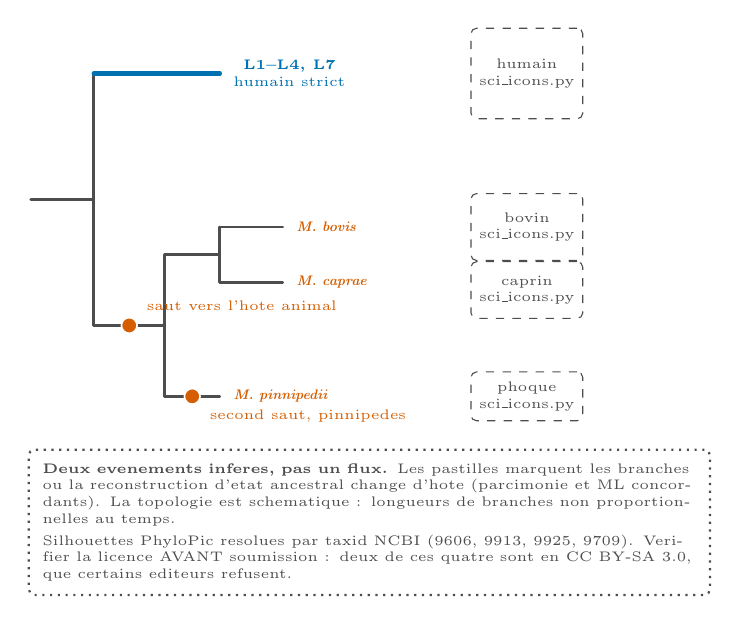
\begin{tikzpicture}[
    every node/.style={font=\scriptsize, align=center},
    br/.style={line width=1pt, color=ng, cap=round},
    brhum/.style={line width=1.6pt, color=humanblue, cap=round},
    tip/.style={font=\tiny\bfseries, anchor=west, inner sep=2pt},
    jump/.style={-{Latex[length=5pt]}, line width=1.2pt, shorten >=3pt, shorten <=3pt},
    ev/.style={circle, fill=animorange, draw=white, line width=0.6pt, inner sep=2pt}
  ]

  % ---- squelette phylogenetique (schematique, non a l'echelle) ----------
  \draw[br] (0,-2.2) -- (0.8,-2.2);
  \draw[br] (0.8,-0.6) -- (0.8,-3.8);
  \draw[brhum] (0.8,-0.6) -- (2.4,-0.6);
  \draw[br] (0.8,-3.8) -- (1.7,-3.8);
  \draw[br] (1.7,-2.9) -- (1.7,-4.7);
  \draw[br] (1.7,-2.9) -- (2.4,-2.9);
  \draw[br] (1.7,-4.7) -- (2.4,-4.7);
  \draw[br] (2.4,-2.55) -- (2.4,-3.25);
  \draw[br] (2.4,-2.55) -- (3.2,-2.55);
  \draw[br] (2.4,-3.25) -- (3.2,-3.25);

  % ---- feuilles, chacune avec sa silhouette d'hote ----------------------
  \node[tip, text=humanblue] (lh)  at (2.5,-0.6)  {L1--L4, L7\\{\tiny\mdseries humain strict}};
  \node[tip, text=animorange] (lb) at (3.3,-2.55) {\emph{M. bovis}};
  \node[tip, text=animorange] (lc) at (3.3,-3.25) {\emph{M. caprae}};
  \node[tip, text=animorange] (lp) at (2.5,-4.7)  {\emph{M. pinnipedii}};

  \node[inner sep=0pt] at (6.3,-0.6)  {\hosticon{human}{1.15cm}{humain}};
  \node[inner sep=0pt] at (6.3,-2.55) {\hosticon{cattle}{0.85cm}{bovin}};
  \node[inner sep=0pt] at (6.3,-3.35) {\hosticon{goat}{0.72cm}{caprin}};
  \node[inner sep=0pt] at (6.3,-4.7)  {\hosticon{seal}{0.62cm}{phoque}};

  % ---- les evenements de changement d'hote, PLACES SUR LES BRANCHES ----
  % Une pastille par evenement INFERE, jamais une fleche par paire d'hotes :
  % sinon la figure suggere un flux continu la ou il y a deux evenements.
  \node[ev] (e1) at (1.25,-3.8) {};
  \node[ev] (e2) at (2.05,-4.7) {};
  \node[font=\tiny, text=animorange, anchor=west] at (1.35,-3.55) {saut vers l'hote animal};
  \node[font=\tiny, text=animorange, anchor=west] at (2.15,-4.95) {second saut, pinnipedes};

  % ---- encart : ce que la figure affirme, et ce qu'elle ne dit pas -----
  \node[draw=ng, dotted, thick, rounded corners=2pt, inner sep=5pt,
        text width=8.3cm, font=\tiny, align=left, text=ng]
    at (4.3,-6.3)
    {\textbf{Deux evenements inferes, pas un flux.} Les pastilles marquent les branches ou la
     reconstruction d'etat ancestral change d'hote (parcimonie et ML concordants). La topologie
     est schematique : longueurs de branches non proportionnelles au temps.
     \\[2pt]
     Silhouettes PhyloPic resolues par taxid NCBI (9606, 9913, 9925, 9709).
     Verifier la licence AVANT soumission : deux de ces quatre sont en CC BY-SA 3.0,
     que certains editeurs refusent.};

\end{tikzpicture}
\end{document}
